\documentclass[conference]{IEEEtran}

\usepackage[cmex10]{amsmath}
\usepackage{xcolor}

\usepackage{graphicx}
\hyphenation{op-tical net-works semi-conduc-tor}


\begin{document}
\title{Week 2 Report\\ECE 432 Microwave Circuit Design II}

\author{\IEEEauthorblockN{Jackson Pugh}
\IEEEauthorblockA{Portland State University\\
Portland, OR 97207\\
Email: japugh@pdx.edu}
\and
\IEEEauthorblockN{Michael Woodruff}
\IEEEauthorblockA{Portland State University\\
Portland, OR 97207\\
Email: michael.woodruff@pdx.edu}}
\maketitle



\IEEEpeerreviewmaketitle


\section{Introduction}
This lab involves measuring a SAV 541+ transistor from MiniCircuits and obtaining the transfer characteristic curves.  The results obtained in the lab agree very well with the manufacturer's data.
\section{Questions \& Answers}
1. Make nice plots of items 1-2 above. For item 1 comment on how well it compares with specs. For item two, plot the I-V curve but also calculate gm (transconductance) and overlay it. Comment on the dependence of gm on IDS. What are the pros and cons of trying to maximize gm?\\\\\\

\begin{figure}[!h]
\centering
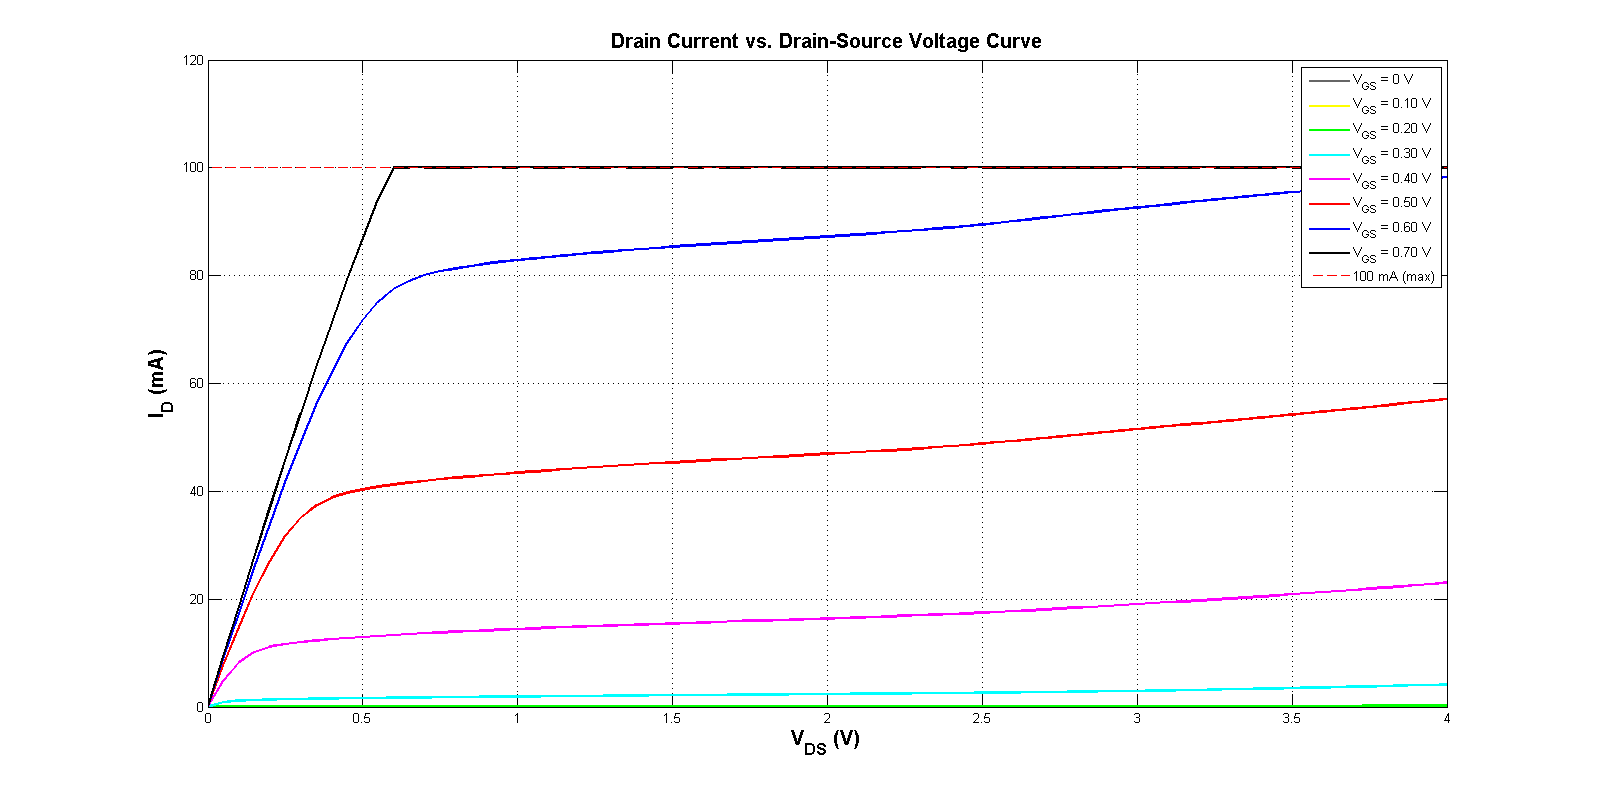
\includegraphics[scale=0.2]{pics/idvsvdds.png}
\caption{$I_{D}$ vs. $V_{DS}$ Curve}
\label{fig:idvsvds}
\end{figure}
\begin{figure}[!h]
\centering
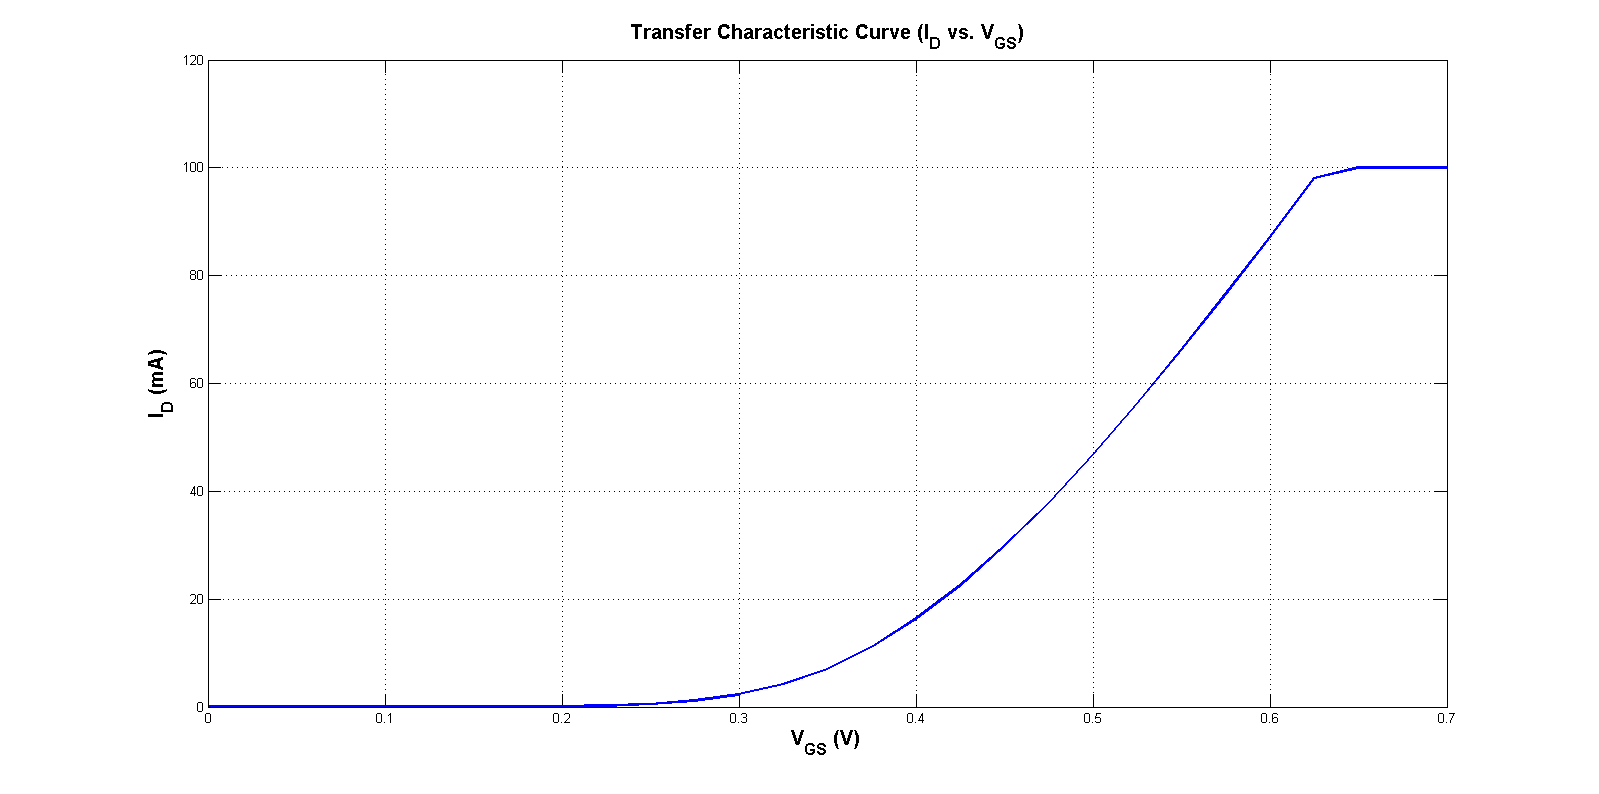
\includegraphics[scale=0.2]{pics/transfercurve.png}
\caption{Transfer Characteristic}
\label{fig:transfercurve}
\end{figure}

\textcolor{red}{Comparing Figure~\ref{fig:idvsvds} against the manufacturer specs shows a fairly significant difference between the drain current for a given drain-source voltage.\\\\
The relationship between $g_m$ and $I_{DS}$ are given by the following equation:
\begin{equation}
g_m = \frac{2I_{DS}}{V_{GS}-V_{T}} 
\end{equation}
The pros of maximizing gm is higher current gain (acts more like an amplifier).  The main tradeoff to this is higher power consumption and more heat dissipation.}\\\\\\
2. For items 3 and 4 compare measured data with S-parameters provided by the company (it's in Touchstone format). Do it separately for all four S parameters and use dB plots for magnitude. For S11 and S22 also plot Smith chart and compare the two results.\\\\\\

\begin{figure}[!h]
\centering
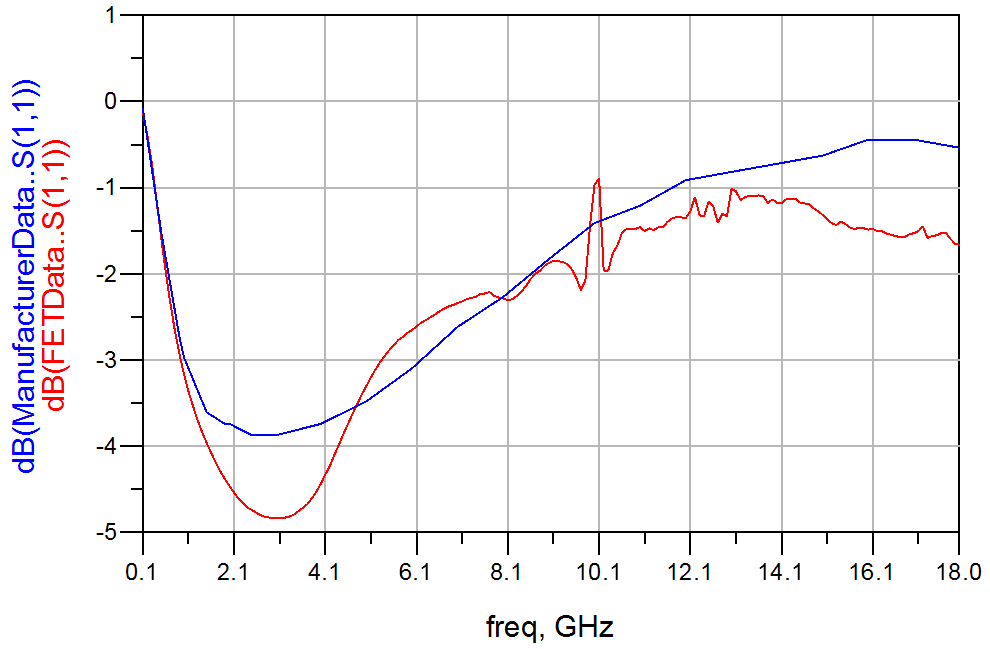
\includegraphics[scale=0.3]{pics/S11Magnitude.png}
\caption{S11 Magnitude}
\label{fig:s11mag}
\end{figure}

\begin{figure}[!h]
\centering
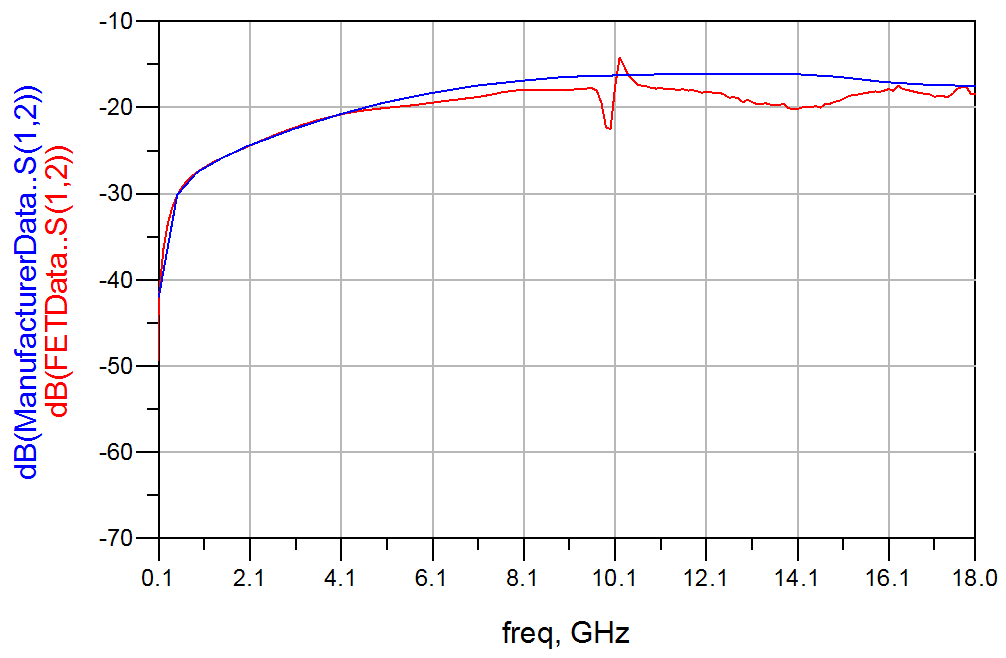
\includegraphics[scale=0.3]{pics/S12Magnitude.png}
\caption{S12 Magnitude}
\label{fig:s12mag}
\end{figure}

\begin{figure}[!h]
\centering
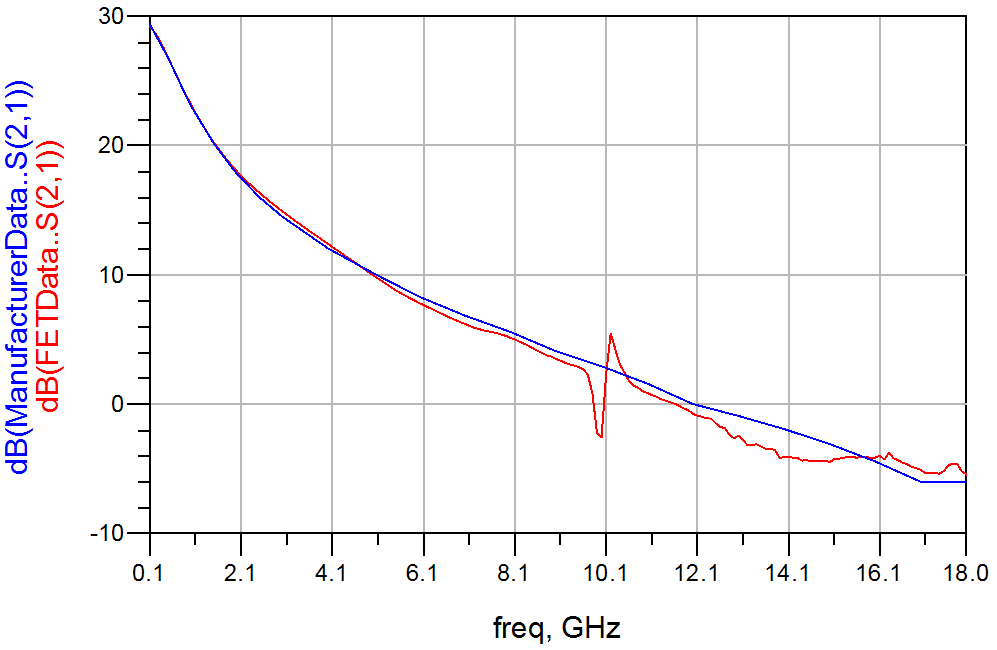
\includegraphics[scale=0.3]{pics/S21Magnitude.png}
\caption{S21 Magnitude}
\label{fig:s21mag}
\end{figure}

\begin{figure}[!h]
\centering
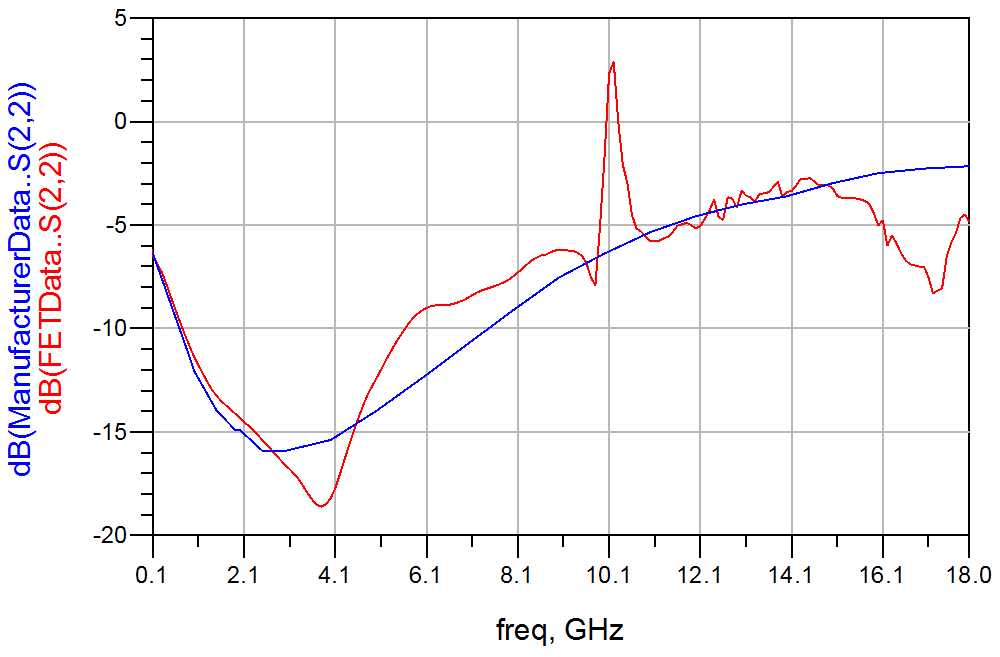
\includegraphics[scale=0.3]{pics/S22Magnitude.png}
\caption{S22 Magnitude}
\label{fig:s22mag}
\end{figure}

\begin{figure}[!h]
\centering
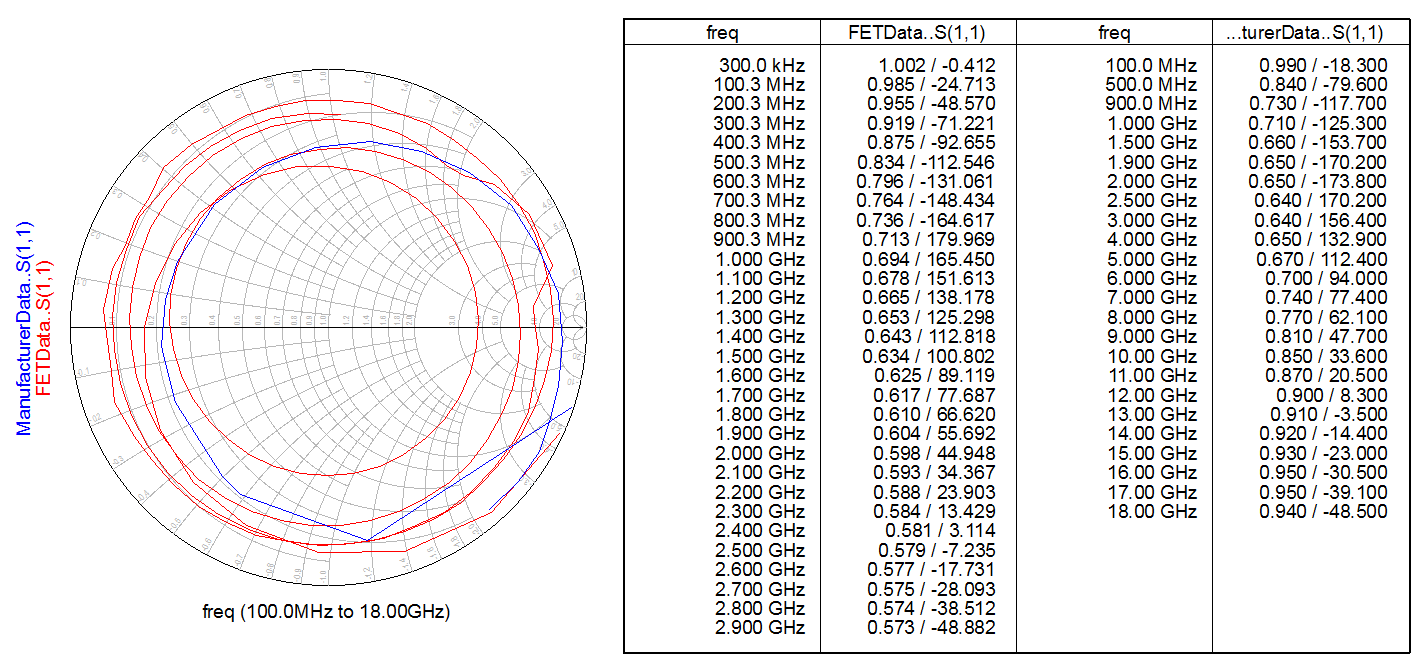
\includegraphics[scale=0.2]{pics/S11Smith.png}
\caption{S11 Smith Plot Before Deembedding}
\label{fig:s11smith}
\end{figure}

\begin{figure}[!h]
\centering
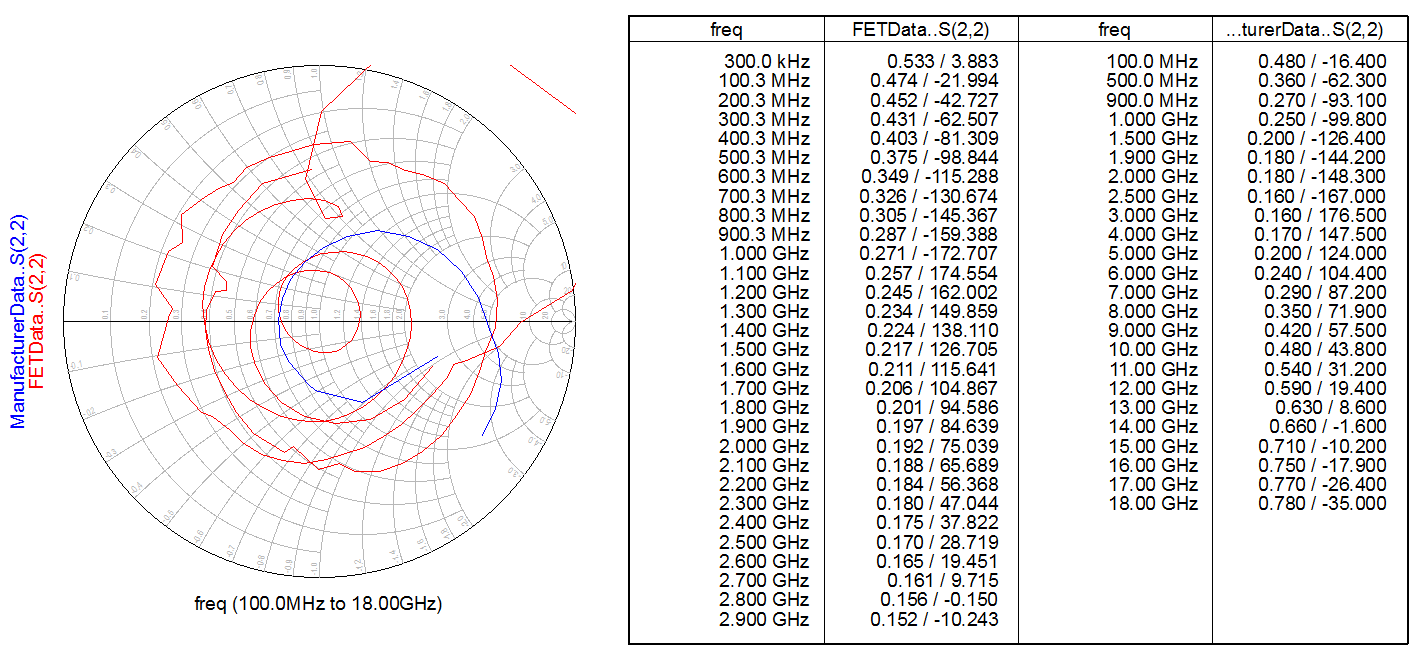
\includegraphics[scale=0.2]{pics/S22Smith.png}
\caption{S22 Smith Plot Before Deembedding}
\label{fig:s22smith}
\end{figure}

\textcolor{red}{The measurements from the lab matched the manufacturer figures well\footnote{There was an abnormal glitch noticed at 10 GHz}.  Looking at the S11 and S22 Smith Charts (see Figure~\ref{fig:s11smith} and Figure~\ref{fig:s22smith}) gave poor results.  This is most likely due to interference caused by the test fixture; deembedding the data may help clean this up.}\\\\\\
3. Measure S-parameters for the fixture and try to use our deembedding procedure from 431/531. Comment on whether this improves the data overall and comparison with manufacturer's data? (for this we may have to de-solder some parts first)\\\\\\

\begin{figure}[!h]
\centering
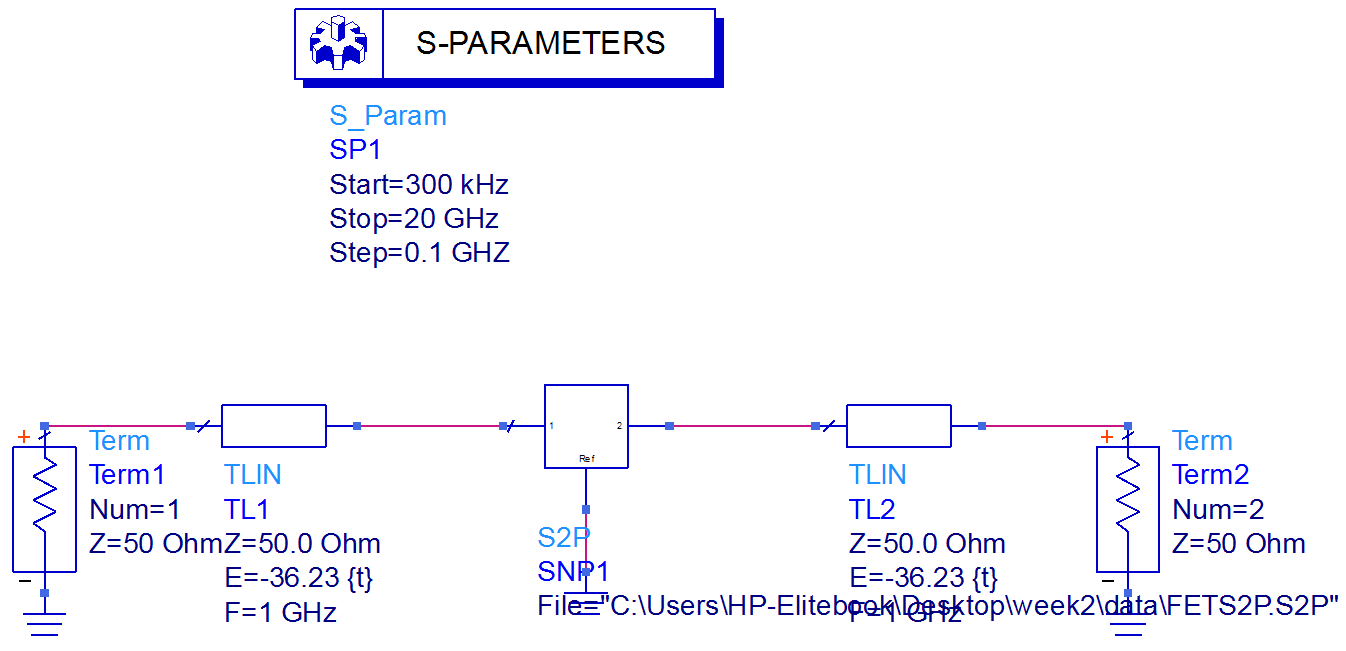
\includegraphics[scale=0.25]{pics/DeembedCircuit.png}
\caption{ADS Deembedding Circuit}
\label{fig:adsdeembed}
\end{figure}
\begin{figure}[!h]
\centering
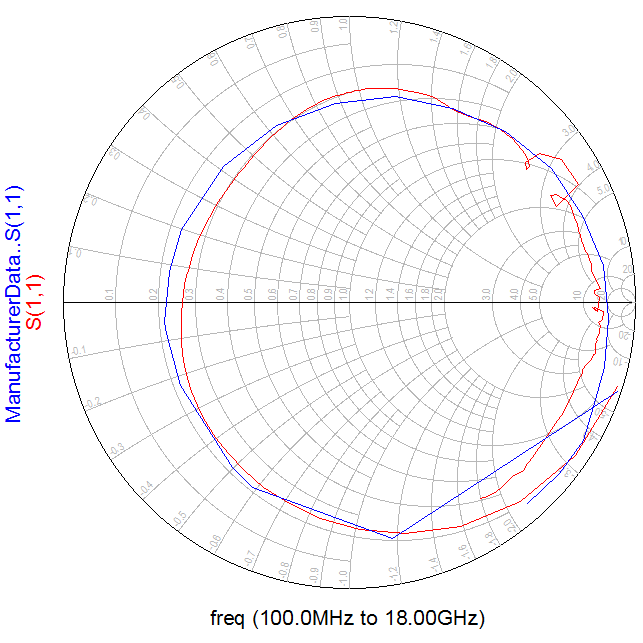
\includegraphics[scale=0.3]{pics/S11SmithDeembed.png}
\caption{S11 Smith Plot After Deembedding}
\label{fig:s11smithdeembed}
\end{figure}
\begin{figure}[!h]
\centering
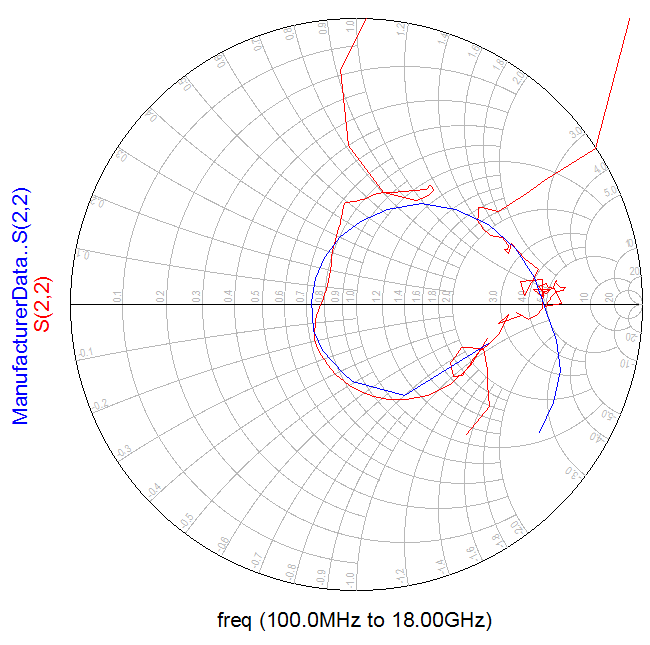
\includegraphics[scale=0.3]{pics/S22SmithDeembed.png}
\caption{S22 Smith Plot After Deembedding}
\label{fig:s22smithdeembed}
\end{figure}

\textcolor{red}{Figure~\ref{fig:adsdeembed} shows the circuit used to deembed the lab measurement data.  The optimal electrical length was around -36.23 degrees for both sides (the test fixture exhibited symmetrical properties).  Looking at the deembedded S11 Smith plot (see Figure~\ref{fig:s11smithdeembed}) showed that deembedding worked well; the S22 Smith plot (Figure~\ref{fig:s22smithdeembed}) has some weird issues that are most likely a glitch in ADS\footnote{I have no idea how to interpret what is going on in the S22 Smith plot simulated from the ADS data}?}
\\\\\\
4. Try to replicate $|$S21$|$ and MSG/MAG plots from manufacturer’s specs; comment on agreement.\\\\\\

\begin{figure}[!h]
\centering
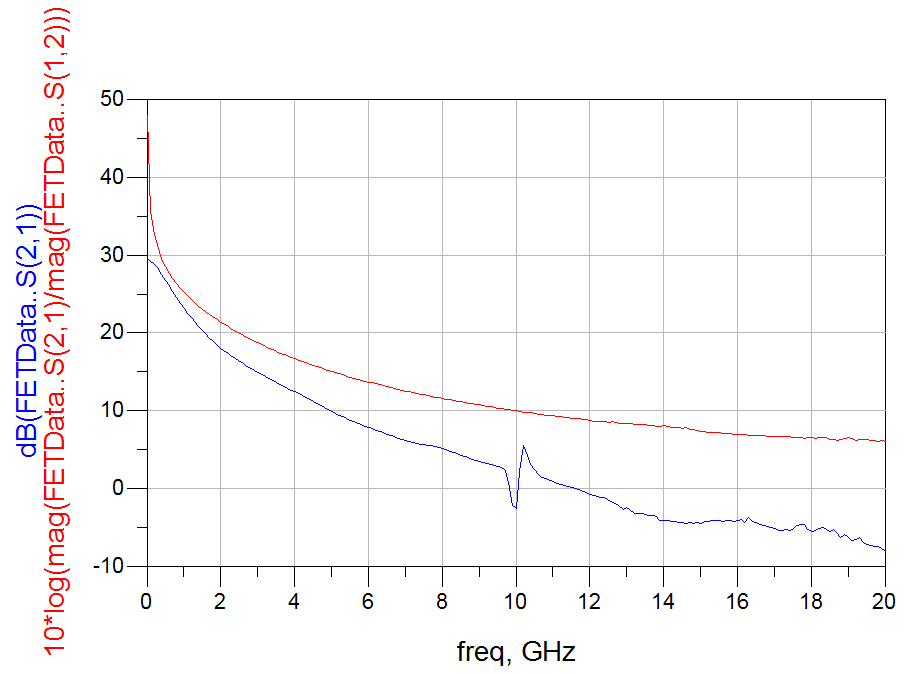
\includegraphics[scale=0.3]{pics/MSGPlot.png}
\caption{$|S_{21}|$ and MSG/MAG Plot Generated From Lab Measurement}
\label{fig:msgplot}
\end{figure}

\textcolor{red}{Figure~\ref{fig:msgplot} shows the replicated $|S_{21}|$ and MSG/MAG plot from the in-lab measurement data.  It matches the manufacturer's specs extremely closely.  This indicates the test setup and measurements were done correctly\footnote{Props to Dr. B and Lunan for nicely setting up and measuring the transistor circuit}.}

\section{Weekly Lessons}
\subsection{In-Class}
Stability and MSG/MAG: In lecture and from the lab, I learned about the maximum available/stable gain (MAG/MSG) and the stability factor K.  Notably, when K is greater than one, the amplifier is unconditionally stable; when K is less than one it is potentially unstable.
\subsection{Outside of Class}
INA vs. Op Amps\cite{IEEEhowto:kopka}: This article examined key differences between instrumentation amplifiers (INA) and op amps.  Some notable things were that INA generally contains internal feedback (as opposed to external, RLC-based feedback) and has minimal external-setting resistors.  In addition, INAs are specifically used in applications demanding high differential-gain and common-mode rejection characteristics.  INAs are designed this way to better amplifiy the signal and reject any common-mode component.  The article discussed a few topologies and analyzed the advantages/disadvantages (e.g. input/output resistance, CMR, and differential gain).  Overall, building an INA using discrete op amps, while fully possible, will not have the desired performance characteristics as that of a monolothic INA.
\begin{thebibliography}{1}
\bibitem{IEEEhowto:kopka}
http://electronicdesign.com/power/what-s-difference-between-operational-amplifiers-and-instrumentation-amplifiers
\end{thebibliography}
\end{document}